\section{Задача синтеза управлений при неопределенности}

Рассмотрим систему
\begin{equation}\label{problem}
    \dot{x} = A(t)x(t) + B(t)u(t) + C(t)v(t)
\end{equation}
с непрерывными матрицами \( A(t), B(t), C(t) \). 
Здесь 
\begin{itemize}
    \item \( x \in \mathbb{R}^n \) --- вектор состояния системы, 
    \item \( u \in \mathbb{R}^p \) --- управление, 
    \item \( v \in \mathbb{R}^q \) --- неизвестное внешнее возмущение,
\end{itemize}
на которые почти всюду по \( t \) наложены некоторые "геометрические"  \ 
 ограничения:
\begin{equation}\label{problem_bounds}
    u(t) \in \mathcal{P}(t), \quad v(t) \in \mathcal{Q}(t),
\end{equation}
 где \( \mathcal{P}(t) \) и \( \mathcal{Q}(t) \) --- заданные непрерывные по \( t \) 
 многозначные функции с выпуклыми компактными значениями. 
Управление может быть выбрано в одном из двух классов:
\begin{itemize}
    \item в классе \( U \) программных управлений u = u(t) --- измеримых по
     Лебегу функций со значениями в \( \mathcal{P}(t) \) почти всюду.
    \item в классе \( U_\mathcal{P} \) позиционных управлений, представляющих
     собой многозначные функции \( \mathcal{U}(t,x) \subseteq
     \mathcal{P}(t) \). При этом выполнены условия существования и
     продолжаемости решения дифференциального включения
    \begin{equation}\label{dif_inclusion}
        \dot{x} \in A(t)x + B(t)\mathcal{U}(t,x) + C(t)v(t), \quad
         t_0 \le t \le t_1, 
    \end{equation}
    для любой измеримой по Лебегу функции \( v(t) \). \footnote{Примером класса
     \( U_\mathcal{P} \) может служить класс всех непрерывных по \( t \) и
     полунепрерывных сверху по \( x \) многозначных отображений с выпуклыми
     компактными значениями. В этом случае дифференциальное включение имеет
     решение на всем отрезке времени для произвольного \( x^0 = x(t_0) \),
     то есть существует абсолютно непрерывная функция \( x(t) \),
     удовлетворяющая дифференциальному включению почти всюду.} Далее речь пойдет
     именно про этот тип управлений, как наиболее пригодный для решения задач с 
     неопределенностью.
\end{itemize}
Важно отметить, что в задачах с неопределенностью эти два типа управлений
 существенно не взимозаменяемы. Имея позиционное управление, подстановкой его
 и решением задачи относительно \( u(t) \), уже нельзя однозначно найти
 программный аналог. Перейдем к постановке задачи синтеза управлений при 
 неопределенности.

Пусть задано "целевое" \ множество \( \mathcal{M} \in \text{comp} \,
 \mathbb{R}^n \). Задача о синтезе управлений при неопределенности состоит 
 в отыскании множества разрешимости \( \mathcal{W}(\tau, t_1, \mathcal{M}) = 
 \mathcal{W}[\tau] \) и позиционной стратегии управления
 \( \mathcal{U}(t,x) \in U_{\mathcal{P}} \) таких, что все решения
 \eqref{dif_inclusion}, выпущенные из любой начальной позиции \( \{\tau, 
 x_{\tau}\}, \, x_{\tau} = x(\tau), \, x_{\tau} \in \mathcal{W}(\tau, t_1, 
 \mathcal{M}), \, \tau \in [t_0, t_1) \), достигали бы целевого множества
 \( \mathcal{M} \) в момент времени \( t_1 \) при любом внешнем возмущении
 \( v(t) \in \mathcal{Q}(t) \). То есть для данного целевого множества и 
 геометрических ограничений на управление и помеху необходимо найти трубку
 разрешимости, состоящую их всех состояний системы в различные моменты времени
 \( t \), для которых вне зависимости от помехи существовала бы некоторая 
 стратегия управления, приводящая систему в требуемое множество. Также 
 для каждого такого состояния необходимо отыскать соответствующее целевое 
 управление. Очевидно, что задача имеет смысл в случае
 \( \mathcal{W}(\tau, t_1, \mathcal{M}) \ne \varnothing \).
 
Многозначная функция \( \mathcal{W}[t] = \mathcal{W}(t, t_1,\mathcal{M}) \) 
 называется трубкой разрешимости или мостом Красовского. Далее будет показано,
 что трубка разрешимости может быть представлена в виде некоторого многозначного
 интеграла, который называют альтернированным интегралом Л.С. Понтрягина.

\section{Альтернированный интеграл Понтрягина}
Для начала приведем исходную систему \eqref{problem} к более простому виду.
 Для этого сделаем невырожденную замену \( x(t) = G(t_1, t)x(t) \), где 
 \( G(t,t_1) \) --- фундаментальная матрица однородного уравнения 
 \eqref{problem}. В таком случае система примет вид:
\begin{equation}\label{simplified_problem}
    \dot{x} = u + v,
\end{equation}
 а ограничения на управление и помеху изменятся:
\begin{equation}\label{simplified_bounds}
 \begin{gathered}
    u \in \mathcal{P}_0(t), \quad v \in \mathcal{Q}_0(t); \\
    \mathcal{P}_0(t) = G(t_1, t) B(t) \mathcal{P}(t), \, \mathcal{Q}_0 = 
     G(t_1,t)C(t)\mathcal{Q}(t).
 \end{gathered}
\end{equation}
Далее вместо \eqref{problem} с ограничениями \eqref{problem_bounds} будем 
 рассматривать \eqref{simplified_problem} с ограничениями \eqref{simplified_bounds},
 опуская индекс нуль.

Естественно было бы определенить множество разрешимости двумя способами в терминах
 максимина и минимакса. Начнем с первого из них.

 \begin{definition}
    Множеством разрешимости максиминного типа назовем множество
    \begin{equation*}
        W[\tau] = W(\tau, t_1, \mathcal{M}) = \left\{ x: \, \max_v \min_u
         d^2(x(t_1), \mathcal{M}) \le 0 \mid x(\tau) = x \right\}, 
    \end{equation*}
     где \( d^2(x. \mathcal{M}) = \min\limits_z \{ (x-z,x-z) \mid z \in 
     \mathcal{M} \} \) и \( x(t_1) \) --- конец в момент \( t_1 \) траектории
     \( x(t) \) системы \eqref{simplified_problem}, выпущенной из положения 
     \( x(\tau) = x \) при некоторых \( u(\cdot) \in U \) и \( v(t) \in 
     \mathcal{Q}(t) \).
\end{definition}

Такое множество имеет аналитическое представление, а именно справедливо
 утверждение:

\begin{statement}
    Для \( W[t] \) справедливо представление:
    \begin{equation}\label{solvability_set_format}
        W(t,t_1,\mathcal{M}) = \left( \mathcal{M} + \int\limits_t^{t_1} 
         (-\mathcal{P}(t)) dt \right) \dot{-} \int\limits_t^{t_1} \mathcal{Q}(t) dt,
         \quad \tau \le t \le t_1.
    \end{equation}
    Здесь символ \( \mathcal{P} \dot{-} \mathcal{Q} \) означает геометрическую
     разность двух множеств \( \mathcal{P}, \, \mathcal{Q}\). А именно,
     \( c \in \mathcal{P} \dot{-} \mathcal{Q} \) тогда и только тогда, когда \(c +
     \mathcal{Q} \subseteq \mathcal{P} \).
\end{statement}
\begin{proof}
    При заданных \( u, v \) на интервале \( (t, t_1 ) \) значение на правом конце
     выражается как 
    \begin{equation*}
        x(t_1) = x(t) + \int\limits_t^{t_1}u(\tau)d\tau + \int\limits_t^{t_1}
        v(\tau)d\tau.
    \end{equation*}
    В таком случае множество разрешимости в терминах объединений и пересечений 
     представляется в виде
    \begin{multline*}
        W(t, t_1, \mathcal{M}) = \bigcap\limits_{v \in \mathcal{Q}} 
         \bigcup\limits_{u \in \mathcal{P}} \left\{ x : x = x(t_1)
         -\int\limits_t^{t_1}u(\tau) d\tau - \int\limits_t^{t_1} v(\tau)
         d\tau, \, x(t_1) \in \mathcal{M} \right\} = \\
        = \bigcap\limits_{v \in \mathcal{Q}} \bigcup\limits_{u \in 
         \mathcal{P}} \left\{ \mathcal{M} - \int\limits_t^{t_1} u(\tau) d\tau
         - \int\limits_t^{t_1} v(\tau) d\tau \right\} = \\
        = \bigcap\limits_{v \in \mathcal{Q}} \left\{ \mathcal{M} +
         \int\limits_t^{t_1}(-\mathcal{P}(\tau)) d\tau - \int\limits_t^{t_1}
         v(\tau) d\tau \right\} = \\
        = \left\{ x : x \in \left( \mathcal{M} + \int\limits_t^{t_1}(- \mathcal{P}
         (\tau)) \right)  - \int\limits_t^{t_1} v(\tau) d\tau, \, \forall v(\tau)
         \in \mathcal{Q}(\tau) \right\} = \\
        = \left\{ x : x + \int\limits_t^{t_1} v(\tau) d\tau \in \mathcal{M} + 
         \int\limits_t^{t_1}(- \mathcal{P}(\tau)) d\tau, \, \forall v(\tau) \in
         \mathcal{Q}(\tau) \right\}.
    \end{multline*}
    Последнее в силу определения геометрической разности совпадает 
     \eqref{solvability_set_format}.
\end{proof}

Опишем процедуру последовательного построения альтернированного интеграла. Взяв
 интервал \( \tau \le t \le t_1 \), рассмотрим его разбиение \( \Sigma_k = \{ \sigma_1,
 \dots, \sigma_k \} \),
\begin{equation*}
    t = t_1 - \sum_{i=1}^k \sigma_i, \dots, t_1 - \sigma_1, t_1, \quad \sigma_i > 0.
\end{equation*}
На первом шаге, найдем множество \( W[t_1 - \sigma_1] = 
 W(t_1 - \sigma_1, t_1, \mathcal{M}) \). Вследствие \eqref{solvability_set_format}
 будем иметь
\begin{equation*}
     W(t_1 - \sigma_1, t_1, \mathcal{M}) = \left( \mathcal{M} + \int\limits_{t_1 - \sigma_1}
     ^{t_1}(-\mathcal{P}(\tau)) d\tau \right) \dot{-} \int\limits_{t_1 - \sigma_1}^{t_1}
     \mathcal{Q}(\tau)d\tau.
\end{equation*}
В следующей точке разбиения, имея в виду уже построенное на предыдущем шаге множество получим
\begin{equation*}
    \begin{gathered}
        W(t_1 - \sigma_1 -\sigma_2, t_1 - \sigma_1, W[t_1 - \sigma_1]) = \left( W[t_1 - \sigma_1]
        + \int\limits_{t_1 - \sigma_1 - \sigma_2}^{t_1 - \sigma_1} (-\mathcal{P}(\tau))d\tau \right)
        \dot{-} \\
        \dot{-} \int\limits_{t_1 - \sigma_1 - \sigma_2}^{t_1 - \sigma_1} \mathcal{Q}(\tau) d\tau
    \end{gathered}
\end{equation*}
Продолжая процедуру, на левом конце получим множество разрешимости в виде суперпозиции множеств, 
 построенных для всех предыдущих точек разбиения:
\begin{equation*}
    W(t, t + \sigma_k, W(t + \sigma_k, t + \sigma_k + \sigma_{k-1}, \dots, W(t_1 - \sigma_1, t_1,
    \mathcal{M}))) = \mathcal{I}(t, t_1, \mathcal{M}, \Sigma_k).
\end{equation*}
Для корректного построения предполагается, что все возникающие здесь множества непусты. Это может 
 быть обеспечено следующим предположением:
\begin{assumption}\label{assumption_nonempty}
    Существует такая непрерывная функция \( \beta(t) > 0, \, t \in [t_0, t_1] \), что все
     множества
    \begin{equation}
        \begin{gathered}
            W \left( t_1 - \sum_{i=1}^j\sigma_i, t_1 - \sum_{i = 1}^{j - 1}\sigma_i, W 
             \left( t_1 - \sum_{i = 1}^ {j - 1} \sigma_1, t_1 - \sum_{i = 1}^{j - 2} 
             \sigma_i, \dots, W(t_1 - \sigma_1, t_1, \mathcal{M}) \right) \dots \right)
             \dot{-} \\
            \dot{-} \ \beta \left( t_1 - \sum_{i = 1}^j \sigma_i
             \right) S \ne \varnothing 
        \end{gathered}
    \end{equation}
    при \( j = 1, \dots, k \), каким бы ни было разбиение \( \Sigma_k \).
\end{assumption}

Ниже всюду будем считать предположение \eqref{assumption_nonempty} выполненым. Отметим,
 что данное предположение важно и без него дальнейшие утверждения могут быть неверны.

Следуя приведенной схеме, приходим к аналитическому выражению для "дискретного" \ множества
 разрешимости.
 
\begin{multline}\label{pontr_analytical}
    \mathcal{I}(t, t_1, \mathcal{M}, \Sigma_k) = \left( \dots \left( \left( \mathcal{M} + 
     \int\limits_{t_1 - \sigma_1}^{t_1} (-\mathcal{P}(\tau)) d\tau \right) \dot{-} \int\limits_
     {t_1 - \sigma_1}^{t_1} \mathcal{Q}(\tau) d\tau \right) + \dots \dot{-} \right. \\
    \left. \int\limits_t^{t + \sigma_k} \mathcal{Q}(\tau) d\tau \right).
\end{multline}

При этом множества \( \mathcal{I} (t, t_1, \mathcal{M}, \Sigma_k) \) есть выпуклые компакты 
 для любого разбиения \( \Sigma_k \).

Для дальнейшего напомним определение хаусдорфова расстояния между выпуклыми компактными 
 множествами.

\begin{definition}
    Хаусдорфово полурасстояние между компактами \( \mathcal{Q}, \mathcal{M} \)
    определяется как 
    \begin{equation*} 
        h_+(\mathcal{Q}, \mathcal{M}) = \max_x \min_z \{(x - z, x - z)^{1/2} \mid x \in \mathcal{Q}, 
        z \in \mathcal{M} \},
    \end{equation*}
    в то время как хаусдорфово расстояние:
    \begin{equation*}
        h(\mathcal{Q}, \mathcal{M}) = \max \{ h_+(\mathcal{Q}, \mathcal{M}), 
         h_+(\mathcal{M}, \mathcal{Q}) \}.
    \end{equation*}
\end{definition}
        
Оказывается, что для построенных выше множеств \( \mathcal{I}(t, t_1, \mathcal{M}, \Sigma_k) \), при измельчении
 рассмотренного разбиения, существует хаусдорфов предел, не зависящий от 
 разбиения \( \Sigma_k \) (См. например \cite{lin_dif_chasing}). Это наталкивает на мысль о том,
 что этот предел является действительным множеством разрешимости задачи \eqref{simplified_problem}.

\begin{lemma}\label{lemma_haus_limit}
    Существует хаусдорфов предел \( \mathcal{I}(t, t_1, \mathcal{M}) \)
    \begin{equation*}
        \lim h \left( \mathcal{I}(t, t_1, \mathcal{M}, \Sigma_k), \mathcal{I}(t, t_1, \mathcal{M})
         \right) = 0
    \end{equation*}
    при 
    \begin{equation*}
        \max\{\sigma_i: i = 1,\dots, k \} \to 0, \quad k \to \infty, \quad \sum_{i = 1}^k \sigma_i 
         = t_1 - t. 
    \end{equation*}
    Этот предел не зависит от способа разбиения \( \Sigma_k \).
\end{lemma}
Множество \( \mathcal{I}(t, t_1, \mathcal{M}) \) будем называть \emph{альтернированной областью 
 разрешимости} задачи \eqref{simplified_problem}. Фактически множество \( \mathcal{I}(t, t_1, 
 \mathcal{M}) \) есть значение некоторого многозначного интеграла, известного как 
 \emph{альтернированный интеграл Понтрягина}. Будем обозначать его как

\begin{equation}
    \mathcal{I}(t, t_1, \mathcal{M}) = \int\limits_{t_1, \mathcal{M}}^t \left( (-\mathcal{P}(\tau))
     d\tau \dot{-} \mathcal{Q}(\tau) d\tau \right).
\end{equation}


\begin{lemma}\label{lemma_semigroup_property}
    Многозначное отображение \( \mathcal{I}(t, t_1, \mathcal{M}) \) удовлетворяет полугрупповому
     свойству:
    \begin{equation}
        \mathcal{I}(t, t_1, \mathcal{M}) = \mathcal{I}(\tau, t, \mathcal{I}(t, t_1,\
         \mathcal{M})), \quad  \tau \le t \le t_1.
    \end{equation}
\end{lemma}
\begin{proof}
    Доказательство этого факта вытекает из свойства аддитивности альтернированного интеграла,
     которое доказывается, например, в \cite{lin_dif_chasing}.
\end{proof}

Ключевое свойство альтернированного интеграла содержит следующая 
\begin{theorem}
    Множество разрешимости \( \mathcal{W}[t] \) может быть представлено как 
    \begin{equation}
        \mathcal{W}[t] \equiv \mathcal{I}(t, t_1, \mathcal{M}), \quad
         t_0 \le t \le t_1.
    \end{equation}
\end{theorem}

Аналогично построению альтернированного интеграла, исходящему из понятия множества разрешимости
 максиминного типа, возможно по аналогичной последовательной схеме построить альтернированный
 интеграл второго рода. Выясняется, что построенные при этом множества разрешимости совпадают
 и равны действительному множеству разрешимости задачи.

Прежде чем приступить к аналогичной процедуре построения альтернированного инеграла второго рода
дадим необходимое определение.

\begin{definition}
    Множество разрешимости \( W^-[\tau] \) минимаксоного типа называется следующая совокупность
     векторов
    \begin{equation*}
        W_-[\tau] = W_-(\tau, t_1, \mathcal{M}) = \{ x : \min_u \max_v d^2(x(t_1),
         \mathcal{M}) \le 0 \mid x(\tau) = x \}.
    \end{equation*}
\end{definition}
Для введенного множества справедливо представление аналогичное представлению 
 \eqref{solvability_set_format}.
\begin{statement}
    Для \( W_-[\tau] \) справедливо представление
    \begin{equation}
        W_-(\tau, t_1, \mathcal{M}) = \left( \mathcal{M} \dot{-} \int\limits_{\tau}^{t_1}
         \mathcal{Q}(t) dt \right) + \int\limits_{\tau}^{t_1} (-\mathcal{P}(t)) dt, \quad 
         t_0 \le s \le t_1.
    \end{equation}
\end{statement}
Доказательство этого утверждения проводится аналогично доказательству соответствующего утверждения для
 множества максиминного типа.

Теперь, аналогично построению альтернированного интеграла Понтрягина \( \mathcal{I}(\tau, t_1,
 \mathcal{M}) \), рассмотрим суперпозицию множеств \( W_-(t, t_1, \mathcal{M}) \) для произвольного
 разбиения \( \Sigma_k = \{ \sigma_1, \dots, \sigma_k\} \) отрезка \( \tau \le t \le t_1 \).

\begin{equation*}
    W_-(t_1 - \sigma_1, t_1, \mathcal{M}) = \left( \mathcal{M} \dot{-} \int\limits_{t_1 - 
     \sigma_1}^{t_1} \mathcal{Q}(s) ds \right) + \int\limits_{t_1 - \sigma_1}^{t_1} (-\mathcal{P}(s))ds.
\end{equation*}
И далее приходим к выражению
\begin{multline}\label{}
    \mathcal{I}_-(t, t_1, \mathcal{M}, \Sigma_k) = \left(\dots\left(\left(\mathcal{M} \dot{-}
     \int\limits_{t_1 - \sigma_1}^{t_1} \mathcal{Q}(\tau) d\tau \right) + \int\limits_{t_1 - 
     \sigma_1}^{t_1}(-\mathcal{P}(\tau)) d\tau \right) \dot{-} \dots \right. \\
    \left. + \int\limits_{t}^{t + \sigma_k} (-\mathcal{P}(\tau))) d\tau \right) .
\end{multline}

Здесь, как и прежде, предполгается, что возникающие множества не пусты. Для этого примем
\begin{assumption}\label{assumption_nonempty_2}
    Для произвольного разбиения существует непрерывная функция \( g(t) : [t_0, t_1] \to \mathbb{R}^n \)
     и числа \( r_j \) такие, что
    \begin{equation*}
        g \left(t_1 - \sum_{i = 1}^j \sigma_i \right) + r_j B \subseteq \mathcal{I}_-\left[ t_1 - 
         \sum_{i = 1}^j \sigma_i \right], \quad j = 1, \dots, m.
    \end{equation*}
\end{assumption}

Для построенных таким образом множеств справедливо утверждение аналогичное лемме \eqref{lemma_haus_limit}

\begin{lemma}
    Существует хаусдорфов предел \( \mathcal{I}_-(\tau, t_1, \mathcal{M}) \)
    \[
        \lim h \left( \mathcal{I}_-(\tau, t_1, \mathcal{M}, \Sigma_k), \mathcal{I}_-(\tau, t_1,
         \mathcal{M}) \right) = 0    
    \]
    при
    \[
        \max\{\sigma_i : i = 1, \dots, k \} \to 0, \quad k \to \infty, \quad \sum_{i = 1}^k 
         \sigma_i = t_1 - \tau,
    \]
    и этот предел не зависит от выбора разбиений \( \Sigma_k \).
\end{lemma}

Будем называть \( \mathcal{I}_-(\tau, t_1, \mathcal{M}) \) \emph{альтернированным 
 интегралом Понтрягина второго рода}.

Можно заметить, что альтернированные интегралы разных типов соответствуют различным 
 информационным схемам. Альтернированный интеграл Понтрягина предполагает появление 
 информации о помехах с опережением, а интеграл второго рода --- с запаздыванием. 
 Замечательно, что при условиях невырожденности \eqref{assumption_nonempty} и 
 \eqref{assumption_nonempty_2} в пределе эти схемы дают один и тот же результат, а именно,
 справедливо утверждение.

\begin{theorem}
    Альтернированный интеграл Понтрягина совпадает с альтернированным интегралом второго рода:
    \begin{equation*}
        \mathcal{I}(t, t_1, \mathcal{M}) = \mathcal{I}_-(t, t_1, \mathcal{M}).
    \end{equation*}
\end{theorem}

Из вышесказанного можно сделать вывод, что множество разрешимости системы имеет явный вид и
 представляется в виде альтернированного интерала, который можно считать дискретными методами,
 зная опорные функции множеств в него входящих. Трудность в таком подходе возникает при попытке
 подсчитать опорную функцию разности двух множеств, которая вообще говоря удовлетворяет
\begin{equation*}
    \rho(l \mid A \dot{-} B) = \text{conv}( \rho(l \mid A) - \rho(l \mid B)) \le \rho(l \mid A) -
      \rho(l \mid B), \quad \forall l \in \mathbb{R}^n.
\end{equation*}
В связи с этим возникает необходимость весьма трудоемкого "овыпукления" \ разности опорных функций.
Рассмотренный далее подход эллипсоидальных аппроксимаций позволяет избежать этой проблемы.

\section{Функции цены}
Применительно к данной задаче, рассмотрим подход к решению с помощью функций цены. Введем

\begin{equation*}
    \mathcal{V} = \min_{\mathcal{U}} \max_{x(\cdot)} \{\mathcal{I}(t,x) \mid \mathcal{U} \in 
     U_{\mathcal{P}}, \, x(\cdot) \in \mathcal{X}_{\mathcal{U}}(\cdot) \}.
\end{equation*}
Здесь функционал
\begin{equation*}
     \mathcal{I}(t,x) = d^2(x[t_1], \mathcal{M}),
\end{equation*}
а \( \mathcal{X}_{\mathcal{U}}(\cdot) \) --- множество всех траекторий дифференциального включения
\begin{equation*}
    \dot{x} \in \mathcal{U}(t,x) + \mathcal{Q}(t), \quad x(\tau) = x,
\end{equation*}
порожденных стратегией \( \mathcal{U} \in U_{\mathcal{P}} \).

Для введенной функции \( \mathcal{V}(t,x) \) можно составить уравнение Гамильтона-Якоби-Беллмана-Айзекса:
\begin{equation}\label{HJBI}
    \frac{\partial \mathcal{V}}{\partial t} + \min_u \max_v \left( \frac{\partial \mathcal{V}}
     {\partial x}, u + v \right) = 0, \quad u \in \mathcal{P}(t), \ v \in \mathcal{Q}(t),
\end{equation}
с граничным условием
\begin{equation}\label{HJBI_boundary}
    \mathcal{V}(t_1, x) = d^2(x, \mathcal{M}).
\end{equation}

Аналогично введенным выше рекуррентным схемам построения альтернированных интегралов, 
введем рекуррентную схему построения функций цены. Как и ранее рассмотрим интервал 
 \( \tau \le t \le t_1 \) и построим его разбиение \( \Sigma_k = \{ \sigma_1, \dots, \sigma_k \} \).
 Для этого разбиения рассмотрим соотношения:
\begin{equation*}
    V_k^+(t_1 - \sigma_1, x) = \left\{ \max_v \min_u d^2(x(t_1), \mathcal{M}) \mid t_1 -
     \sigma_1 \le t \le t_1, \ x(t_1 - \sigma_1) = x \right\},
\end{equation*}
\begin{multline*} 
    V_k^+(t_1 - \sigma_1 - \sigma_2, x) = \left\{ \max_v \min_u V_k^+(t_1 - \sigma_1, x(t_1 -
     \sigma_1)) \mid t_1 - \sigma_1 - \sigma_2 \le t \le t_1 - \sigma_1, \right. \\ 
    x(t_1 - \sigma_1 - \sigma_2) = x \Big\}.
\end{multline*}
Продолжая процедуру, в точке \( \tau = t_1 - \sum\limits_{i = 1}^k \sigma_i \) получаем:
\begin{equation*}
    V_k^+(\tau, x) = \left\{ \max_v \min_u V_k^+ (\tau + \sigma_k, x(\tau + \sigma_k)) \mid
     \tau \le t \le \tau + \sigma_k, \ x(\tau) = x \right\},
\end{equation*}
Всюду будем предполагать, что "максимины" \ существуют.

Оказывается, что для введенных таким образом функций, при неограниченном измельчении разбиения,
 существуют поточечные пределы, то есть справедлива

\begin{lemma}
    При
    \begin{equation*}
        \max_{i = 1,\dots,k} \{\sigma_i\} \to 0, \quad k \to \infty, \quad \sum_{i = 1}^k \sigma_i = 
         t_1 - \tau, 
    \end{equation*}
    существует поточечный предел
    \begin{equation*}
        V^+(\tau, x) = \lim_{k \to \infty} V_k^+(\tau, x),
    \end{equation*}
    не зависящий от выбора разбиения \( \Sigma_k \).
\end{lemma}
Будем называть \( V^+(\tau, x) \) \emph{последовательным максимином}.
\begin{lemma}
    Функция \( V^+(\tau, x) \) удовлетворяет полурупповому свойству
    \[
        V^+(\tau, x \mid V^+(t_1, \cdot)) = V^+(\tau, x \mid V^+(t, \cdot \mid V^+(t_1, 
         \cdot))).  
    \]
    При этом справедливо неравенство
    \[
        V^+(t, x) \ge \left\{ \max_v \min_u V^+(t + \sigma, x(t + \sigma)) \mid x(t) = x 
         \right\}, \quad \sigma > 0.
    \]
\end{lemma}

Отметим связь функции с альтернированным интегралом.
\begin{lemma}
    Справедливо равенство
    \[
        V^+ (\tau, x) = d^2(x, \mathcal{W}^*(\tau, t_1, \mathcal{M})),
    \]
    где \( \mathcal{W}^*[\tau] = \mathcal{W}^*(\tau, t_1, \mathcal{M}) = \mathcal{I}(\tau,
     t_1, \mathcal{M}) \) --- значение альтернированного интеграла
\end{lemma}
Отюсда прямо следует
\begin{lemma}
    Альтернированный инетграл \( \mathcal{I}(\tau, t_1, \mathcal{M}) \) совпадает с
     множеством уровня последовательного максимина \( V^+(\tau, x) \):
    \[
        \mathcal{I}(\tau, t_1, \mathcal{M}) = \{ x : V^+(\tau, x) \le 0 \}.
    \]
\end{lemma}

Теперь рассмотрим задачу аналогичную предыдущей. Для произвольного \( \Sigma_k \), построим
 рекуррентные соотношения 
\begin{equation*}
    V_k^-(t_1 - \sigma_1, x) = \left\{ \min_u \max_v  d^2(x(t_1), \mathcal{M}) \mid t_1 -
     \sigma_1 \le t \le t_1, \ x(t_1 - \sigma_1) = x \right\},
\end{equation*}
\begin{multline*} 
    V_k^-(t_1 - \sigma_1 - \sigma_2, x) = \left\{ \min_u \max_v  V_k^-(t_1 - \sigma_1, x(t_1 -
     \sigma_1)) \mid t_1 - \sigma_1 - \sigma_2 \le t \le t_1 - \sigma_1, \right. \\ 
    x(t_1 - \sigma_1 - \sigma_2) = x \Big\},
\end{multline*}
и так далее. Наконец в точке \( \tau = t_1 - \sum\limits_{i = 1}^k \sigma_i \):
\begin{equation*}
    V_k^-(\tau, x) = \left\{ \min_u \max_v  V_k^- (\tau + \sigma_k, x(\tau + \sigma_k)) \mid
     \tau \le t \le \tau + \sigma_k, \ x(\tau) = x \right\}.
\end{equation*}
Для определенных таким образом функций имеют место аналогичные утверждения
\begin{lemma}
    1. При
    \[ 
        \max_{i = 1,\dots,k} \{\sigma_i\}, \quad k \to \infty, \quad \sum_{i = 1}^k \sigma_i = 
         t_1 - \tau, 
    \]
    существует поточечный предел
    \[
        V^-(\tau, x) = \lim_{k \to \infty} V_k^-(\tau, x),
    \]
    не зависит от выбора разбиения \( \Sigma_k \). \\
    2. Функция \( V^-(\tau, x) \) удовлетворяет полугрупповому свойству.
    \begin{equation}
        V^-(\tau, x \mid V^-(t_1, \cdot)) = V^-(\tau, x \mid V^-(t, \cdot \mid V^-(t_1, \cdot))).
    \end{equation} \\
    3. Справедливо неравенство
    \begin{equation}
        V^-(t,x) \le \min_u \max_v \{ V^-(t + \sigma, x(t + \sigma)) \mid x(t) = x \}, 
         \quad \sigma > 0.
    \end{equation}
\end{lemma}


\begin{lemma}
    Справедливы соотношения:
    \[
        V^-(\tau, x) = d^2(x, \mathcal{W}_-(\tau, t_1, \mathcal{M})),
        \mathcal{I}(\tau, t_1, \mathcal{M}) = \left\{ x : V^-(\tau, x) \le 0 \right\} 
    \]
\end{lemma}

\begin{lemma}
    Многозначное отображение \( \mathcal{W}^-(t, t_1, \mathcal{M}) \) удовлетворяет полугрупповому
     свойству, а именно
    \[
        \mathcal{W}_-(\tau, t_1, \mathcal{M}) = \mathcal{W}_-(\tau, t, \mathcal{W}_-(t, t_1,
         \mathcal{M})), \quad \tau \le t \le t_1.
    \]

\end{lemma}


\section{Решение задачи синтеза}
Суммируем основыне утверждения в виде следующей теоремы.
\begin{theorem}
    1. Последовательные максимин \( V^+(\tau, x) \) и минимакс \( V^-\) равны и совпадают с функцией
     цены \( \mathcal{V}(\tau,x) \):
    \[
        V^+(\tau, x) \equiv V^-(\tau, x) \equiv \mathcal{V}(\tau, x),
    \]
    2. Множество разрешимости задачи допускает следющие эквивалентные представления:
    \[
        \mathcal{I}(\tau, t_1, \mathcal{M}) = \mathcal{W}^*[\tau] = \{ x : \mathcal{V}(\tau \le 0 \},
         \quad t_0 \le \tau \le t_1.
    \]
    То есть, алтернированный интеграл Понтрягина \( \mathcal{I}(\tau, t_1, \mathcal{M}) \), сечение
     моста Красовского \( \mathcal{W}[\tau] \) и множество уровня определенной нами функции
     \( \mathcal{V}(\tau, x) \) суть одно и то же множество. 
\end{theorem}

Кроме того, функция цены \( \mathcal{V}(\tau, x) \) обладает следующими свойствами.
\begin{theorem}
    1. Справедлив принцип оптимальности
    \[
        \mathcal{V}(\tau, x \mid \mathcal{V}(t_1, \cdot)) = \mathcal{V}(\tau, x \mid \mathcal{V}(t, 
         \cdot \mid \mathcal{V}(t_1, \cdot))), \quad \mathcal{V}(t_1, x) \equiv d^2(x, \mathcal{M}),
         \quad \tau \le t \le t_1. 
    \]
    2. Если существует непрерывная частная производная \( \partial \rho(l \mid \mathcal{W}[t]) / 
     \partial t, \forall l \in \mathbb{R}^n \), то фукнция \( \mathcal{V}(t, x) \) является 
     классическим решением уравнения Гамильтона-Якоби-Беллмана-Айзекса.
    \[
        \frac{\partial \mathcal{V}}{\partial t} + \min_u \max_v \left( \frac{\partial \mathcal{V}}
         {\partial x}, u + v \right) = 0
    \]
    с краевым условием \( \mathcal{V}(t_1, x) = h_+^2(x, \mathcal{M}) \).
\end{theorem}

Если решение \eqref{HJBI}, \eqref{HJBI_boundary} удается найти, то гарантирующая стратегия управления
 находится следубщим образом:
\begin{equation}
    \mathcal{U}_*(t,x) = \mathrm{argmin} \left\{ \left( \frac{\partial \mathcal{V}}{\partial x},
     u \right) : u \in \mathcal{P}(t) \right\},
\end{equation}
если градиент \( \partial \mathcal{V} / \partial x \) существует в точке \( (t, x) \). Или в общем
 случае
\begin{equation}
    \mathcal{U}_*(t,x) = \left\{ u: \max_v \{ dh_+^2(x, \mathcal{W}[t]) / dt : v \in \mathcal{Q}(t) \} 
     \le 0 \right\}.
\end{equation}

\begin{theorem}\label{dif_incl_theorem}
    Все решения дифференциального включения
    \begin{equation*}
        \dot{x} \in \mathcal{U}_*(t,x) + v(t), \quad x_{\tau} = x(\tau) \in \mathcal{W}[t],
    \end{equation*}
    удовлетворяют включению \( x(t) \in \mathcal{W}[t] , \tau \le t \le t_1 \), и, следовательно,
     достигают целевого множества \( \mathcal{M} : x(t_1) \in \mathcal{M} \) при любом возмущении
     \( v(t) \). 
\end{theorem}

Таким образом синтезирующая стратегия \( \mathcal{U}_*(t,x) \) разрешает задачу целевого синтеза 
 управлений при неопределенности. Среди допустимых стратегий \( \mathcal{U}(t,x) \), удовлетворяющих
 включению \( \mathcal{U}(t,x) \subseteq \mathcal{U}_*(t,x) \), то есть обеспечивающих выполнение
 теоремы \eqref{dif_incl_theorem}, находится стратегия "экстремального прицеливания" , задаваемая
 условиями
\begin{equation}
    \mathcal{U}_e(t,x) = \partial_l k(t, -l) = \mathrm{arg min} \{(l^0, u) \mid u \in \mathcal{P}(t) \}.
\end{equation}
Здесь \( \partial_l k \) --- субдифференциал функции \( k(t, l) \) по переменной \( l \), \( k(t,l)
 = \rho(l \mid \mathcal{P}(t)), l^0 = l^0(t, x) \ne 0 \) --- максимизатор задачи 
\begin{equation}\label{extr_problem}
    h_+(x, \mathcal{W}[\tau]) = \max \{(l,x) - \rho(l \mid \mathcal{W}[\tau]) \mid (l,l) \le 1 \},
\end{equation}
причем \( l^0(t,x) = 0 \), если \( h_+(x, \mathcal{W}[\tau)) = 0 \).

Как видно для поиска гарантирующей стратегии достаточно знать лишь сечения \( \mathcal{W}[t] \) функции
 цены \( \mathcal{V}(t,x) \). Поскольку интегрирование уравнения Гамильтона-Якоби, как правило, очень 
 нетривиально, будем использовать аппроксимации сечения функции цены вместо самой функции. Таким 
 образом сведем задачу к задаче поиска аппроксимаций альтернированного интеграла Понтрягина.

\section{Эллипсоидальные аппроксимации множества разрешимости}
Будем рассматривать систему
\begin{equation*}
    \dot{x} = u + v
\end{equation*}
с эллипсоидальными ограничениями
\begin{equation*}
    u \in \mathcal{E}(p(t), P(t)), \quad v \in \mathcal{E}(q(t), Q(t)), \quad \mathcal{M} = 
     \mathcal{E}(m, M).
\end{equation*}
Здесь функции \( p(t), q(t), P(t), Q(t) \) предполагаются заданными и непрерывными. Вектор \( m \) и
 матрица \( M \) фиксированы. Эллипсоиды задаются своим центром и матрицей следующим образом:
 
\begin{equation}
    \mathcal{E}(a, Q) = \left\{ x : (x - a, Q^{-1}(x - a)) \le 1 \right\}, \quad x \in \mathbb{R}^n,
\end{equation}
где \( Q > 0 \).

Приведем для начала основные утверждения эллипсоидального исчисления, необходимые в дальнейшем. Подробнее 
см. \cite{ellips_calculus} и \cite{reach_an_unc_sys}.

\begin{theorem}\label{ellips_theorem}
    Пусть \( \mathcal{E}_1(a_1, Q_1), \mathcal{E}_2(a_2, Q_2) \) --- пара невырожденных эллипсоидов. Рассмотрим
    \begin{itemize}
        \item семейство матриц \( Q[p] \):
        \begin{equation*}
            \begin{gathered}
                Q[p] = (1 + p^{-1})Q_1 + (1 + p) Q_2,\\
                p \in \Pi^+ = \left[ \lambda_{\mathrm{min}}^{1/2}, \lambda_{\mathrm{max}}^{1/2} 
                 \right]
            \end{gathered}
        \end{equation*}
        где \( \lambda_{\mathrm{min}} > 0, \lambda_{\mathrm{max}} < \infty \) --- относительные
         собственные
        значения пары матриц \( Q_1, Q_2 \), или, иначе, корни уравнения
        \begin{equation*}
            \det (Q_1 - \lambda Q_2) = 0.
        \end{equation*}
        Обозначим также
        \begin{equation*}
            \Pi^- = \Pi^+ \cap(1, \lambda_{\mathrm{min}})
        \end{equation*}
        \item семейство матриц \( Q[S_1,S_2] \):
        \begin{equation*}
            Q[S_1, S_2] = (S_1 Q_1^{1/2} + S_2 Q_2^{1/2})^T (S_1 Q_1^{1/2} + S_2 Q_2^{1/2}),
        \end{equation*}
        где
        \begin{equation*}
            S_1, S_2 \in \Sigma = \{ S \in \mathcal{L}(\mathbb{R}^n, \mathbb{R}^n): S^T S = S S^T = I \}.
        \end{equation*}
    \end{itemize}
    Для этих семейств справедливы следующие включения:
    \begin{equation}
        \mathcal{E}_1 + \mathcal{E}_2 \supseteq \mathcal{E}(a_1 + a_2, Q[S_1, S_2]), \quad \forall S_1, S_2 \in \Sigma
    \end{equation}
    \begin{equation}
        \mathcal{E}_1 \dot{-} \mathcal{E}_2 \supseteq \mathcal{E}(a_1 - a_2, Q[-p]), \quad \forall p \in \Pi^-
    \end{equation}
\end{theorem}

Более того, для некоторого фиксированного вектора \( l \) представляется возможным найти значения параметров
\( p, S_1, S_2 \) такие, что для опорных функций суммы и разности эллипсоидов и их внутренних оценок справедливо
равенство. Или иначе, внутренняя оценка касается суммы или разности эллипсоидов.

\begin{theorem}
    Для невырожденных эллипсоидов \( \mathcal{E}(a_1, Q_1), \mathcal{E}(a_2, Q_2) \) справедливо:
    \begin{itemize}
        \item Для любого вектора \( l \) существуют значения параметров \( S_1^*, S_2^* \in \Sigma \) такие, что
        \begin{equation*}
            \rho(l \mid \mathcal{E}(a_1, Q_1) + \mathcal{E}(a_2, Q_2)) = \rho(l \mid \mathcal{E}(a_1 + a_2, Q[S_1^*, S_2^*])),
        \end{equation*}
        \item Для всех "хороших" \ направлений \( l \) геометрической разности эллипсоидов существует значение \( p* \in \Pi^- \) такое, что
        \begin{equation*}
            \rho(l \mid \mathcal{E}(a_1, Q_1) \dot{-} \mathcal{E}(a_2, Q_2)) = \rho(l \mid \mathcal{E}(a_1 - a_2, Q[-p*])).
        \end{equation*}
    \end{itemize}
\end{theorem}


Отправной точкой для построения оценок множества разрешимости является тот факт, что функция 
 \( \mathcal{W}[t] \) в условиях невырожденности предположения \eqref{assumption_nonempty} является 
 решением эволюционного уравнения.

\begin{theorem}
    Многозначная функция \( \mathcal{W}[t] \) удовлетворяет при всех \( t \in [t_0, t_1 ]\) 
     эволюционному уравнению
    \begin{equation}\label{evolution_equation}
        \lim_{\sigma \to 0} \sigma^{-1} h_+ \left( \mathcal{W}[t - \sigma], \left( \mathcal{W}[t] - 
         \sigma \mathcal{E}(p(t), P(t)) \right) \dot{-} \sigma \mathcal{E}(q(t), Q(t)) \right) = 0,
         \quad \mathcal{W}[t_1] = \mathcal{M}.
    \end{equation}
    и это решение максимально по включению относительно всех других решений этого уравнения. 
\end{theorem}

При этом мы будем заинтересованы именно во внутренних аппроксимациях множества разрешимости, так как
 построение управления по схеме описанной в следующем разделе, "удерживающее" траекторию внутри такой
 аппроксимации будет гарантировать попадание в целевое множество. Поэтому будем искать максимальное 
 по включению эллипсоидальное решение \eqref{evolution_equation}. Исходя из эволюционного уравнения будем
 строить внутреннюю аппроксимацию, пользуясь формулами из теоремы \eqref{ellips_theorem}. В итоге приходим
 к утверждению

\begin{theorem}
    Эллипсоидозначная функция \( \mathcal{E}_-[t] = \mathcal{E}(x^*, X_-(t)) \), определяемая
     дифференциальными уравнениями:
    \begin{equation}\label{dif_center}
        \dot{x^*}(t) = p(t) + q(t),
    \end{equation}
    а также
    \begin{equation}\label{dif_matrix}
        \begin{gathered}
            \dot{X_-}(t) = \pi(t) X_-(t) + \pi^{-1}(t) Q(t) - \\
             - (X_-(t))^{1/2} H(t) (P(t))^{1/2} - (P(t))^{1/2} H^T(t) (X_-(t))^{1/2}
        \end{gathered}
    \end{equation}
    с краевыми условиями соответственно
    \begin{equation}\label{dif_boundary}
        x(t_1) = m, \quad X_-(t_1) = M.
    \end{equation}
    является решением \eqref{evolution_equation}.
    
    При этом для любого вектора \( l \in \mathbb{R}^n \) сущетсвуют функции \( \pi(t), H(t) \) такие,
     что
    \begin{equation}
        \rho(l \mid \mathcal{W}[t]) = \rho(l \mid \mathcal{E}(x^*, X_-(t | \pi(\cdot), H(\cdot))))
    \end{equation}
    что означает, что построенный эллипсоид \( \mathcal{E} \) является максимальным по включению
     решением \eqref{evolution_equation}. 
\end{theorem}

\section{Эллипсоидальный синтез управлений}
Следуя предыдущим разделам, для вычисления стратегии управления требуется найти множество разрешимости
 \( \mathcal{W}[\cdot] \), определить значение функции цены \( \mathcal{V}(t,x) = d^2(x(t),
 \mathcal{W}(t)) \) и её градиент, решить задачу \eqref{extr_problem}. Для множеств произвольной формы
 все эти задачи, вообще говоря, представляют большую сложность. Поэтому основная идея эллипсоидального
 синтеза состоит в замене \( \mathcal{W}[t] \) некоторой его внутренней эллипсоидальной аппроксимацией,
 и применении вышеописанной схемы к ней. Это даёт:

\begin{equation}\label{control}
    \mathcal{U}_-(t,x) = 
     \begin{cases}
        \mathcal{E}(p(t), P(t)), & \text{если} x \in \mathcal{E}_-[t], \\
        p(t) - P(t)l^0(l^0, P(t)l^0)^{-1/2}, & \text{если} x \notin \mathcal{E}_-[t],
     \end{cases}
\end{equation}
где \( l^0 = l^0(t,x) \) --- единичный вектор, максимизатор задачи
\begin{equation}
    h_+(x, \mathcal{E}_-[t]) = (l^0,x) - \rho(l^0 \mid \mathcal{E}_-[t]) = \max\{(l,x) - \rho(l \mid 
     \mathcal{E}_-[t]) \mid \| l \| \le 1 \}.
\end{equation}

Последняя задача теперь может быть решена однозначно. Если 
\begin{equation}
    s^0 = \text{argmin}\{ \| x - s \| : s \in \mathcal{E}_-[t], x = x(t) \},
\end{equation}
то можно положить \( l^0 = k(x(t) - s^0), k > 0 \), так что вектор \( l^0 \) будет градиентом функции
\( h_+(x, \mathcal{E}_-[t]) \) при фиксированном \( t \). 

\begin{lemma}
    Рассмотрим невырожденный эллипсоид \( \mathcal{E} = \mathcal{E}(x^*, X) \) и вектор \( x \notin 
     \mathcal{E}(x^*, Q). \) Тогда градиент
    \begin{equation*}
        l^0 = \partial h_+(x, \mathcal{E}(x^*, X)) / \partial x
    \end{equation*}
    может быть выражен как 
    \begin{equation}
        l^0 = \frac{x - s^0}{\| x - s^0 \|}, \quad s^0 = (I + \lambda X^{-1})^{-1}(x - x^*) + x^*.
    \end{equation}
    Здесь множитель лагранжа \( \lambda > 0 \) --- единственный корень уравнения \( f(\lambda) = 0 \),
    где
    \begin{equation*}
        f(\lambda) = ((I + \lambda X^{-1})^{-1}(x - x^*), X^{-1}(I + \lambda X^{-1})^{-1}(x - x^*)) - 1.
    \end{equation*}
\end{lemma}

При этом понятно, что при известных \( x^*, X \) параметр \( \lambda \) может быть представлен 
 единственным образом как \( \lambda = \lambda(x) \).

Выражение для управления \eqref{control} является следствием следующего факта:
\begin{lemma}
    Пусть задан эллипсоид \( \mathcal{E}(p, P) \). Тогда минимизатор \( u^* \) задачи
    \begin{equation*}
        \min\{ (l^0, u) \mid u \in \mathcal{E}(p, P)) \} = (l, u^*), \quad l \ne 0, 
    \end{equation*}
    есть вектор \( u^* = p - Pl(l, Pl)^{-1/2} \).
\end{lemma}

\section{Пример синтеза гарантирующего управления}

\subsection{Пример 1}
Будем рассматривать ту же систему
\begin{equation*}
    \dot{x} = u + v
\end{equation*}
с эллипсоидальными ограничениями:
\begin{gather*}
    \mathcal{M} = \mathcal{E}(m, M), \quad
    m = \begin{bmatrix}
        0 \\[0.3em]
        0
    \end{bmatrix}, \quad
    M = \begin{bmatrix}
        1 & 0 \\[0.3em]
        0 & 1
    \end{bmatrix}, \\
    \mathcal{P} = \mathcal{E}(p, P), \quad
    p = \begin{bmatrix}
        0 \\[0.3em]
        0
    \end{bmatrix}, \quad
    P = \begin{bmatrix}
        2 & 0 \\[0.3em]
        0 & 1
    \end{bmatrix}, \\
    \mathcal{Q} = \mathcal{E}(q, Q), \quad
    q = \begin{bmatrix}
        0 \\[0.3em]
        0
    \end{bmatrix}, \quad
    Q = \begin{bmatrix}
        1 & 0 \\[0.3em]
        0 & 1
    \end{bmatrix}. \\
\end{gather*}
Начальное условие для траекторий:
\begin{equation*}
    x_0 = \begin{bmatrix}
        -0.3 \\[0.3em]
        -0.3
    \end{bmatrix}.
\end{equation*}
Помеху выберем например как
\begin{equation*}
    v(t) = \begin{bmatrix}
        sin(t) \\[0.3em]
        cos(t)
    \end{bmatrix}.
\end{equation*}


Визуализируем полученную оценку для дискретной схемы (Рис. \eqref{fig:inner_tube}). 
Построим график оценки и траектории. Траектория, упираясь в границу эллипсоидальной трубки,
 идет по этой границе, так как генерирующееся управления стремится оставить её внутри
 эллипсоидальной оценки. Как итог траектория приходит в целевое множество.

\begin{figure}[ht]
	\centering
	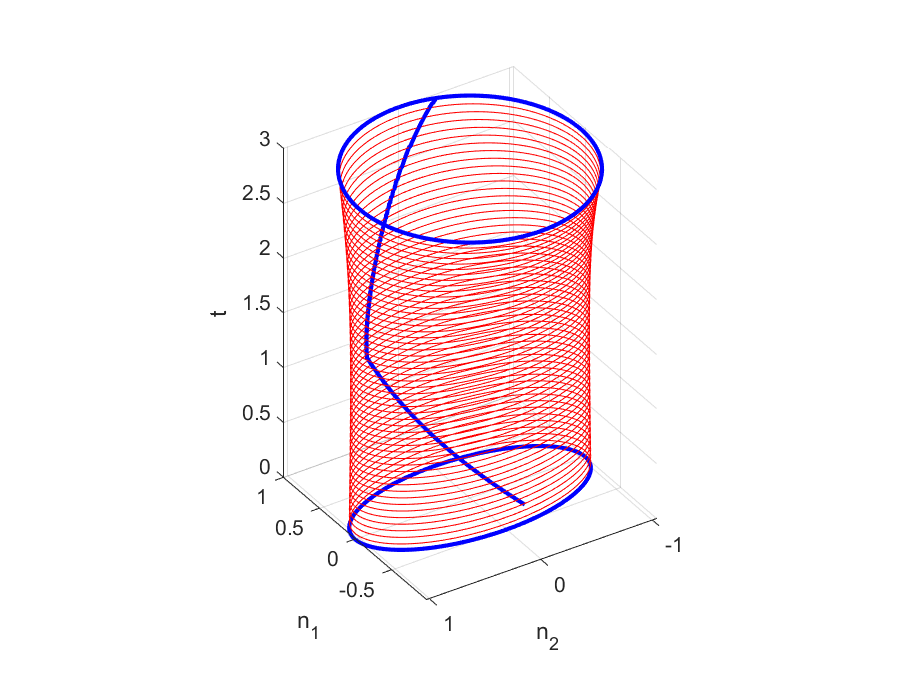
\includegraphics[width = 0.9\linewidth]{"./resources/solv_tube.pdf"}
	\caption{Внутренняя эллипсоидальная оценка для множества разрешимости и траектория системы.}
    \label{fig:inner_tube}
\end{figure}

\subsection{Пример 2}
\begin{equation*}
    \dot{x}(t) = u(t) + v(t),
\end{equation*}
где на управление и помеху наложены эллипсоидальные ограничения:
\begin{gather*}
    \mathcal{M} = \mathcal{E}(m, M), \quad
    m = \begin{bmatrix}
        0 \\[0.3em]
        0
    \end{bmatrix}, \quad
    M = \begin{bmatrix}
        1 & 0 \\[0.3em]
        0 & 1
    \end{bmatrix}, \\
    \mathcal{P}(t) = \mathcal{E}(p(t), P(t)), \quad
    p(t) = \begin{bmatrix}
        0 \\[0.3em]
        0
    \end{bmatrix}, \quad
    P(t) = \begin{bmatrix}
        sin(3t) + 2 & 0 \\[0.3em]
        0 & sin(3t) + 2
    \end{bmatrix}, \\
    \mathcal{Q}(t) = \mathcal{E}(q(t), Q(t)), \quad
    q(t) = \begin{bmatrix}
        0 \\[0.3em]
        0
    \end{bmatrix}, \quad
    Q(t) = \begin{bmatrix}
        cos(3t) + 2 & 0 \\[0.3em]
        0 & cos(3t) + 2
    \end{bmatrix}. \\
\end{gather*}
Начальное условие для траекторий:
\begin{equation*}
    x_0 = \begin{bmatrix}
        0 \\[0.3em]
        0
    \end{bmatrix}.
\end{equation*}
Помеху выберем например следующим образом:
\begin{equation*}
    v(t) = \begin{bmatrix}
        sin(t) \\[0.3em]
        cos(t)
    \end{bmatrix}.
\end{equation*}
В этом примере ограничения на управление и помеху поочередно "доминируют" \ друг на другом, поэтому соответствующий альтернированный интеграл
 с течением времени расширяется и сужается.

\subsection{Особенности численного метода}

Для численного решения задач и удобной визуализации будем использовать язык
 Matlab. Из теоретической части ясно, что для задач с эллипсоидальными ограничениями
 эллипсоидальные трубки разрешимости удовлетворяют дифференциальным уравнениям \eqref{dif_center}
 и  \eqref{dif_matrix} с конечными условиями \eqref{dif_boundary}.
Для решения подобных дифференциальных уравнений удобно пользоваться итерационными 
 методами. Будем использовать классический метод Эйлера.
Разобьем отрезок времени на \( n \) частей: \( t_0 < t_1 < t_2 < \dots < t_{n-1} < t_n \). 
 Для каждого момента, начиная с \( t_n \), последовательно определим центр \( x^*(t_k) \) внутренней
 эллипсоидальной трубки и матрицу \( X_-(t_k) \). 

Важно отметить, что в \eqref{dif_matrix} в виде параметров присутствуют
 функции \( \pi(t) > 0 \) и \( H(t) \). На каждом шаге
 решения дифференциальных уравнений будем определять значения параметров, так, чтобы внутренняя оценка
 касалась действительного множества разрешимости в некотором выбранном направлении \( l \).
 Для этого будем выбирать ортогональную матрицу \( H(t) \) из соотношения
\begin{equation*}
    H(t)(P(t))^{1/2} l = \frac{\langle l, P(t) l \rangle^{1/2}}{\langle l, X_-(t) l \rangle^{1/2}} (X_-(t))^{1/2} l.
\end{equation*}
Такую матрицу можно найти с помощью сингулярного разложения векторов
\begin{equation*}
    v = (P(t))^{1/2} l, \quad w = \frac{\langle l, P(t) l \rangle^{1/2}}{\langle l, X_-(t) l \rangle^{1/2}} (X_-(t))^{1/2} l.
\end{equation*}
А значение \( \pi(t) \) как
\begin{equation*}
    \pi(t) = \frac{\langle l(t), Q(t) l(t) \rangle^{1/2}}{\langle l(t), X_-(t) l(t) \rangle^{1/2}}.
\end{equation*}

Отметим также, что гарантированно построить управление в задаче можно, если начальное положение
 системы \( x(t_0) = x_0 \) принадлежит эллипсоиду \( \mathcal{E}(x^*(t_0), X_-(t_0)) \), 
 поэтому это условие необходимо проверить. В таком случае для каждого момента времени \( t_k \), имея
 центр \( x^*(t_k) \) и матрицу \( X_-(t_k) \) внутренней оценки, возможно по приведенной теоретической
 схеме построить управление в точках введенной сетки.

\begin{equation*}
    u(t_k, x) = \begin{cases}
        p(t_k), & \text{если} \ x \in \mathcal{E}(x^*(t_i), X_-(t_i)), \\
        p(t_k) - P(t_k)l^0(l^0, P(t_k)l^0)^{-1/2}, & \text{если} \ x \notin \mathcal{E}(x^*(t_k), X_-(t_k)). 
    \end{cases}
\end{equation*}
Вектор \( l^0 \) в соответствии с теоретической схемой может быть найден как:
\begin{equation}
    l^0 = \frac{x - s^0}{\| x - s^0 \|}, \quad s^0 = (I + \lambda X_-^{-1}(t_k))^{-1}(x - x^*(t_k)) + x^*(t_k).
\end{equation}

Остаётся найти значение множителя \( \lambda \), которое можно искать из уравнения \( f(\lambda) = 0 \), где
\begin{equation*}
    f(\lambda) = ((I + \lambda X_-^{-1}(t_k))^{-1}(x - x^*(t_k)), X_-^{-1}(t_k)(I + \lambda X_-^{-1}(t_k))^{-1}(x - x*(t_k))) - 1
\end{equation*}

Очевидно, что если \( x \notin \mathcal{E}(x^*(t_k), X_-(t_k)) \), тогда в точке \( \lambda = 0, \ f(0) > 0 \).
При этом при \( \lambda \to \infty \) имеем
\begin{equation}
    ((I + \lambda Q^{-1})^{-1}x, Q^{-1}(I + \lambda Q^{-1})^{-1}x ) \to 0.
\end{equation}
А также \( f'(\lambda) < 0 \) при  \( \lambda > 0. \) Поэтому значение параметра можно искать итерационно среди 
 \( \lambda > 0 \). 

Траекторию системы таким образом также удобно строить итерационно, исходя из разностого уравнения

\begin{equation*}
    x(t_{k+1}) - x(t_k) = h(u(t_k, x(t_k)) + v(t_k)), \quad h = t_{k+1} - t_k,
\end{equation*}
корректируя управление в точках сетки.

\section{Более общая задача}

Рассмотрим исходную систему
\begin{equation*}
    \dot{x}(t) = A(t) x(t) + B(t) u(t) + C(t) v(t)
\end{equation*}
с эллипсоидальными ограничениями
\begin{equation*}
    u(t) \in \mathcal{E}(p(t), P(t)) \subset \mathbb{R}^p, \quad v(t) \in \mathcal{E}(q(t), Q(t)) \subset \mathbb{R}^q.
\end{equation*}
Пусть также задано некоторое эллипсоидальное целевое множество
\begin{equation*}
    \mathcal{M} = \mathcal{E}(m, M) \subset \mathbb{R}^n.
\end{equation*}
Будем строить гарантирующее управление, приводящее систему из некоторого положения 
\( x_0 \) в момент времени \( t_0 \) в целевое множество \( \mathcal{M} \) в момент времени \( t_1 \). Как было отмечено в теоретической части,
 исходная система заменой \( x(t) = G(t_1, t) x(t) \) приводится к виду
\begin{equation*}
    \dot{x}(t) = \hat{B}(t)u(t) + \hat{C}v(t), \quad t \in [t_0, t_1],
\end{equation*}
где 
\begin{equation*}
    \hat{B}(t) = G(t_1, t)B(t), \ \hat{C}(t) = G(t_1, t) C(t)
\end{equation*}
и
\begin{equation*}
    u(t) \in \mathcal{E}(p(t), P(t)), \ v(t) \in \mathcal{E}(q(t), Q(t)).
\end{equation*}

Для новой системы нужно перейти из состояния \( G(t_1, t_0) x_0 \) в целевое множество \( \mathcal{M} \), остающееся без изменений.

Внутренняя эллипсоидальная оценка для системы такого вида может быть найдена из дифференциальных уравнений, которые строятся
 аналогично \eqref{dif_center}, \eqref{dif_matrix}, с учетом того факта, что  \( A \mathcal{E}(q, Q) = \mathcal{E}(Aq, AQA^T) \).

В итоге получаем уравнение на центр:
\begin{equation*}\label{A_dif_center}
    \dot{x}^*(t) = \hat{B}(t) p(t) + \hat{C}(t) q(t)
\end{equation*}
с начальным условием
\begin{equation*}\label{A_dif_center_bound}
    x^*(t_1) = m,
\end{equation*}
и на матрицу конфигурации:
\begin{gather*}\label{A_dif_matrix}
    \dot{X}_-(t) = \pi(t) X_-(t) + \pi^{-1}(t) \hat{C}(t) Q(t) \hat{C}^T(t) - (X_-(t))^{1/2} H(t) (\hat{B}(t) P(t) \hat{B}^T(t))^{1/2} - \\
     - (\hat{B}(t) P(t) \hat{B}^T(t))^{1/2} H^T(t) (X_-(t))^{1/2}
\end{gather*}
с начальным условием
\begin{equation*}\label{A_dif_matr_bound}
    X_-(t_1) = M.
\end{equation*}
Для выполнения условия касания выберем
\begin{equation*}
    \pi(t) = \frac{\langle l(t), \hat{C}(t) Q(t) \hat{C}^T(t) l(t) \rangle^{1/2}}{\langle l(t), X_-(t) l(t) \rangle^{1/2}},
\end{equation*}
а ортогональную матрицу \( H(t) \) будем искать из соотношения
\begin{equation*}
    H(t)(\hat{B}(t) P(t) \hat{B}(t))^{1/2} l(t) = \frac{\langle l(t), \hat{B}(t) P(t) \hat{B}^T(t) l(t) \rangle^{1/2}}{\langle l(t), X_-(t) l(t) \rangle^{1/2}} (X_-(t))^{1/2} l(t).
\end{equation*}

Если в новых координатах найдена внутренняя эллипсоидальная аппроксимация \( \mathcal{E}_-[t] \) множества разрешимости \( \mathcal{W}[t] \), то
управление может быть аналогично найдено в виде обратной связи
\begin{equation*}
    \mathcal{U}_-(t,x) = 
     \begin{cases}
        p(t), & \text{если} \ x \in \mathcal{E}_-[t], \\
        p(t) - P(t)\hat{B}^T(t)l^0(\hat{B}^T(t)l^0, P(t)\hat{B}^T(t)l^0)^{-1/2}, & \text{если} \ x \notin \mathcal{E}_-[t],
     \end{cases}
\end{equation*}
Строя с помощью такого управления траекторию новой системы и выполняя обратное преобразование, получаем 
траекторию исходной системы.